% Nejprve uvedeme tridu dokumentu s volbami
\documentclass[bc,male,html,dept460]{diploma}				% jednostranny dokument
%\documentclass[bc,female,java,dept460,twoside]{diploma}		% oboustranny dokument
\usepackage{czech}
\usepackage[utf8]{inputenc}
\usepackage{indentfirst}

\sloppy
\hyphenation{Python Pythonu SQLUpdate setFixedFilter}

\tolerance=1
\emergencystretch=\maxdimen
\hyphenpenalty=10000
\hbadness=10000

% Zadame pozadovane vstupy pro generovani titulnich stran.
\Author{Jan Žitník}

\Title{Webová aplikace pro PIM \\ (Personal Information Management)}

\EnglishTitle{Web Application for PIM \\ (Personal Information Management)}

\SubmissionDate{16. dubna 2012}

\PrintPublicationAgreement{true}

\AccessRestriction{Licence GPL}

\Thanks{Rád bych na tomto místě poděkoval všem, kteří mi s~prací pomohli, protože bez nich by tato práce nevznikla.}

\CzechAbstract{Cílem této práce je implementovat webovou aplikaci pro organizaci a~správu osobních dat.
Aplikace je určena pro vytváření poznámek, plánování a orgranizaci událostí.
Součástí aplikace je emailový klient a~RSS čtečka implementovaná jako modul.
Práce popisuje architekturu, tvorbu webového serveru a~uživatelského prostředí ve webovém prohlížeči.
}

\CzechKeywords{Python, JavaScript, PIM, DoJo, PostgreSQL}


\EnglishAbstract{The aim of this thesis is to implement web application for managing personal information.
Application is intended for creating notes, planning and time management. Email client and RSS reader is also implemented as a part of this project. Architecture design as well as implementation of both server and client parts is also described.}

\EnglishKeywords{Python, JavaScript, PIM, DoJo, PostgreSQL}

% Pridame pouzivane zkratky (pokud nejake pouzivame).
\AddAcronym{AJAX}{Asynchronou JavaScript And XML}
\AddAcronym{API}{Application Programming Interface}
\AddAcronym{CSS}{Cascading Style Sheet}
\AddAcronym{DOM}{Document Object Model}
\AddAcronym{GNU}{GNU is Not Unix}
\AddAcronym{GPL}{General Public License}
\AddAcronym{GUI}{Graphical User Interface}
\AddAcronym{HTML}{Hyper Text Markup Language}
\AddAcronym{HTTP}{HyperText Transfer Protocol}
\AddAcronym{IMAP}{Internet Message Access Protocol}
\AddAcronym{JSON}{JavaScript Object Notation}
\AddAcronym{LDAP}{Lightweight Directory Access Protocol}
\AddAcronym{PAM}{Pluggable Authentication Module}
\AddAcronym{PIM}{Personal Information Management}
\AddAcronym{RFC}{Request for Comments}
\AddAcronym{RIA}{Rich Internet Application}
\AddAcronym{RSS}{RDF Site Summary}
\AddAcronym{SMTP}{Simple Mail Transfer Protocol}
\AddAcronym{SQL}{Structured Query Language}
\AddAcronym{URL}{Uniform Resource Locator}
\AddAcronym{UTF}{UCS Transformation Format}
\AddAcronym{WSGI}{Web Server Gateway Interface}
\AddAcronym{XML}{eXtended Markup Language}
\AddAcronym{DHTML}{Dynamic HTML}
\AddAcronym{ISO}{International Organization for Standardization}
\AddAcronym{DBMS}{Database management system}
\AddAcronym{JIT}{Just In Time}







% Zacatek dokumentu
\begin{document}

% Nechame vysazet titulni strany.
\MakeTitlePages

% Asi urcite budeme potrebovat obsah prace.
\tableofcontents
\cleardoublepage	% odstrankujeme, u jednostranneho dokumentu o jednu stranku, u oboustrenneho o dve

% % Jsou v praci tabulky? Pokud ano vysazime jejich seznam.
% % Pokud ne smazeme nasledujici makro.
% \listoftables
% \cleardoublepage	% odstrankujeme, u jednostranneho dokumentu o jednu stranku, u oboustrenneho o dve
% 
% % Jsou v praci obrazky? Pokud ano vysazime jejich seznam.
% \listoffigures
% \cleardoublepage	% odstrankujeme, u jednostranneho dokumentu o jednu stranku, u oboustrenneho o dve
% 
% 
% % Jsou v praci vypisy programu? Pokud ano vysazime jejich seznam.
% \lstlistoflistings
% \cleardoublepage	% odstrankujeme, u jednostranneho dokumentu o jednu stranku, u oboustrenneho o dve
% 


% Zacneme uvodem
\section{Úvod}
\label{sec:uvod}
Každý se už určitě setkal s~problémem cokoliv si zapamatovat, vědět kdy je kde jaká schůzka, nebo zapomněl udělat projekt do školy. V~dnešní době jsou papírové organizéry nejen nepraktické, ale špatně se zálohují, nelze v~nich vyhledávat a~mají další nevýhody.
Proto se jeví jako nejlepší východisko úchovávat svá data elektronicky.

Na internetu lze najít spousty hotových řešení, ať už placených, nebo zdarma. Jen málo z nich je ale použitelných. Mnoho takových služeb je poskytováno v~cloudu a~uživatel neví, kdo má k~jeho údajům přistup a~co se s~nimi na pozadí děje.
Cílem této bakalářské práce je vyvinout systém, který je šířen pod otevřenou licencí, je jednoduše rozšiřitelný a~má zdokumentované API. Právě otevřenost systému umožňuje tvorbu libovolných klientských částí, případně využití v~jiných aplikacích.


První část se zabývá vysvětlením pojmů, teorie a~principů, na kterých aplikace zakládá. Je zmíněn programovací jazyk Python, jeho základní popis včetně WSGI rozhraní. Dále je zmíněn Javascript a~framework DoJo pro tvorbu uživatel\-ských rozhraní v~internetovém prohlížeči.

Druhá část bakalářské práce se zabývá návrhem databáze a~architekturou aplikace, podrobné vysvětlení fungování serverové části a~komunikací s~klientskou aplikací.

Třetí část je věnována podrobnému popisu implementace, popisu vzniklých problémů a~jejich řešení. Detailněji ukazuje strukturu programu a~využití specifických knihoven a~frameworků.


\section{Teoretický rozbor}
\label{sec:teorie}
\subsection{Proč PIM}
Projektů pro PIM existuje spousta, placených i~zdarma, ale při bližším prozkoumání žádný nebyl vyhovující.
Většina takovýchto projektů je realizována jako centralizovaná online služba, nejčastěji v~podobě webové stránky.
Uživatelé tak sice mají jednoduchý přístup, ale takovýto způsob ukládání osobních dat není bezpečný, protože nikdy nelze odhadnout, kdo je majitel serveru a~co s~našimi daty ve skutečnosti provádí. Ukládání firemních a~citlivých dat v~takových službách je tedy nemožné.
Existují sice i~open source aplikace, ale kvalita a~uživatelská přívětivost pokulhává.

Při výběru frameworků a~programovacích jazyků byl kladen důraz na nenáročnost, multiplatformnost pro snadnou přenositelnost napříč operačními systémy a~výslednou kvalitu finální aplikace.

Pro tvorbu grafického uživatelského rozhraní se využívá internetového prohlížeče, který je nainstalován na většině počítačů a~není tedy nutné instalovat další programy. Z~toho plyne snadná použitelnost prakticky kdekoliv.
Internetové prohlížeče lze v~dnešní době využívat pro tvorbu aplikací, které jsou takřka k~nerozeznání od nativní aplikace.
Využívá se k~tomu JavaScript a~AJAX, kdy se načte prázdná stránka a~JavaScript dynamicky vytváří GUI prvky, které umisťuje na stránku.
Při interakci s~uživatelem se stránka nikdy nenačítá znovu (refresh), ale data si stáhne ze serveru ve formátu JSON a~případně překreslí určitou část uživatelského rozhraní. Takové aplikace se často označují jako RIA - Rich Internet Application.

Na serverovou část byl zvolen programovací jazyk Python pro svou přehlednost a~snadné použití. Skripty jsou pak spouštěny webovým serverem (nejčastěji Apache) pomocí rozhraní WSGI. Python je interpretovaný jazyk (často označován jako skriptovací) a~jeho interpreter je dostupný pro většinu operačních systémů.

V závěru je pak shrnut celkový výsledek implementace a architekruty, včetně zhodnocení a plánů do budoucna.

\newpage
\subsection{Funkční požadavky}
Nároky na PIM aplikaci byly kladeny tak, aby byly splněny základní potřeby uživatele. Důležitý je čistý objektový návrh tak, aby vývoj mohl v budoucnu neomezeně pokračovat, aby aplikace byla modulární a bylo možné chybějící funkcionalitu doprogramovat.

Mezi základní funkce patří:
\begin{itemize}
 \item Osobní poznámky/deník - přidávání, úpravy včetně mazání
 \item Seznamy/úkoly - přidávání, výpisy nesplněných úkolů
 \item Události a schůzky - plánování, přehledy v kalendáři, týdenní a měsíční pohledy
 \item Aktuality RSS - stahování RSS novinek
 \item E-Mail zprávy - příjem a elektornická korespondence
 \item Adresář - evidence, neomezený počet kontaktů
\end{itemize}

Úkoly, poznámky a události jsou organizovány pomocí tzv. štítků. Štítek je označení určité položky, obdobně jako kategorie.
Každá položka může mít neomezený počet přiřazených štítků, podle kterých lze pak seskupovat výpisy.



\subsection{JavaScript a~RIA aplikace, DoJo}
% \label{sec:teorie-javascript}
JavaScript je objektově orientovaný programovací jazyk, využívaný při tvorbě webových stránek. Na rozdíl od serverových programovacích jazyků (například Python) sloužících ke generování kódu samotné stránky, JavaScript běží na straně klienta, tedy v~prohlížeči.

JavaScript se používá především pro vytváření interaktivních webových stránek. Příkladem použití mohou být nejrůznější kontroly správného vyplnění formulářů, obrázky měnící se po přejetí myší, rozbalovací menu atd. JavaScript se také často používá k~měření statistik návštěvnosti.

Společně s~jazykem HTML (informační kostrou stránky) a~CSS (formátováním vzhledu stránky) je JavaScript součástí DHTML, souboru technik a~postupů zaměřených na zlepšení uživatelského rozhraní a~zvýšení prožitku z~používání stránek. K~tomu JavaScript využívá tzv. DOM, rozhraní umožňující přistupovat k~jednotlivým prvkům stránky.

JavaScript vyvinula společnost Netscape v~roce 1995 a~v~roce 1998 byl standardizován organizací ISO.
\cite{javascript-definice}

Dojo Toolkit je kolekcí JavaScriptových komponent, které mají pomoci webovému vývojáři. Základem je dojo.js, který obsahuje kolekci „nezbytných“ API pro nejčastější použití a~nabízí celou knihovnu funkcí. Dojo je zcela zadarmo pod duální licencí AFL a~BSD licencí.

Druhou částí DoJo toolkitu je GUI knihovna dijit a~dojox, která poskytuje prvky pro tvorbu uživatel\-ských rozhraní, využívá tříd a~dědičnosti.

\subsection{Python, WSGI}
% \label{sec:teorie-javascript}
Programovací jazyk Python vytvořil Guido van Rossum o~Vánocích roku 1989.
Při své práci v~holandském institutu CWI potřeboval jazyk pro psaní utilit pro distribuovaný operační systém,
jenž skupina, ve které pracoval, vyvíjela.
Měl v~úmyslu vytvořit snadno rozšiřitelný jazyk podobný jazyku ABC a~podporující výjimky.
V~únoru roku 1991 na Usenetu ohlásil první veřejnou verzi Pythonu. 

Dnes je Python široce používán na mnoha místech, kde je potřeba přehledný a~snadno spravovatelný kód.
Používá jej i NASA pro uživatelské rozhraní systému řídícího lety raketoplánů, aplikační server Zope,
originální implementace protokolu BitTorrent, balíčkovací systém Portage v~distribuci Gentoo,
stejně tak instalátor Anaconda pocházející z~RedHat Linuxu a~mnohé jiné větší či menší programové celky. 

Python se vyznačuje poměrně netradiční syntaxí založenou na odsazování.
Taktéž může být pro začátečníka matoucí,
že Python je silně objektový beztypový jazyk s~přístupem podobným spíše Smalltalku nežli "běžným"
objektovým jazykům jako je třeba Java. 

Python je jazyk interpretovaný a~často považovaný za skriptovací, přesto je v~něm možno psát i~docela rozsáhlé programové celky.
 
WSGI (Web Server Gateway Interface) definuje jednoduché a~univerzální rozhraní mezi webovým serverem
a~webovou aplikací nebo frameworkem v~programovacím jazyce Python.
Poslední verze jazyka Python, 3.0, vydaná v~prosinci 2008, je již podporována modulem mod\_wsgi webového serveru Apache.
\cite{svec-letajici-cirkus}

\subsection{PostgreSQL}
% \label{sec:teorie-postgres}
PostgreSQL, často jednoduše Postgres, je objektově-relační databázový systém (ORDBMS).
Vydáván je pod licencí typu MIT a~tudíž se jedná o~free a~open source software.
Stejně jako v~případě mnoha dalších open source programů, PostgreSQL není vlastněn jedinou firmou,
ale na jeho vývoji se podílí globální komunita vývojářů a~firem.

PostgreSQL je primárně vyvíjen pro Linux resp. pro unixové systémy obecně, nicméně existují i~balíčky pro platformu win32.
\cite{postgres-wiki}

\section{Architektura aplikace}
\label{sec:architektura}

Princip aplikace je rozdělení na dvě části - klientská strana,
kterou může zastávat jakákoliv vzdálená aplikace (např. JavaScript aplikace pro dekstop, Java aplikace pro Android)
a~na serverovou aplikaci. Tyto dvě komponenty spolu komunikují předem pevně daným protokolem ve formátu JSON.
To přináší mnoho výhod, např. nezávislost klientské aplikace, 
kterou si kdokoliv může napsat díky veřejnému API - díky tomu je možné vytvořit alternativní nativní aplikace pro mobilní platformy,
případně jiné systémy.

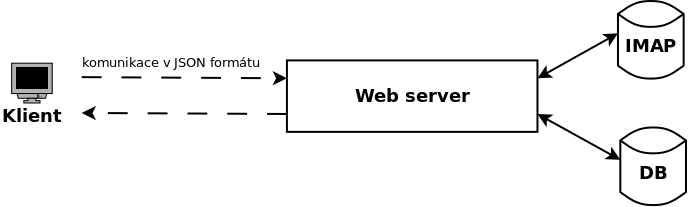
\includegraphics[width=0.7\textwidth]{../applicationArchitecture.png} 

JSON, ve zkratce JavaScript Object Notation je způsob zápisu dat (datový formát) nezávislý na počítačové platformě,
určený pro přenos dat, která mohou být organizována v~polích nebo agregována objektech.
Vstupem je libovolná datová struktura (číslo, řetězec, boolean, objekt nebo z~nich složené pole), výstupem je vždy textový řetězec.
Složitost hierarchie vstupní proměnné není teoreticky nijak neomezena.

Navzdory názvu, JSON je zcela obecný a~může sloužit pro přenos dat (navíc, čitelný pro člověka)
v~libovolném programovacím nebo skriptovacím jazyce.
Data, zapsaná metodou JSON, mohou být samozřejmě uložena a~přenášena v~souborech;
častěji ale přenos probíhá v~prostředí internetu (např. s~použitím technologie AJAX).

Mezi nedostatky JSON patří to, že neumožňuje definovat znakovou sadu přenášeného obsahu,
optimalizace pro přenos binárních dat. Tyto nedostatky platí ale pro některé (slabší) implementace.
Nealfabetické znaky v~řetězcích a~binární data JSON jsou escapovány zpětným lomítkem,
za kterým následuje buď jeden z~běžně používaných znaků (např. $\backslash$n pro nový řádek, $\backslash$t pro tabulátor, $\backslash\backslash$ pro samotné zpětné lomítko) nebo $\backslash$u indikující znak z~Unicode (UTF-16), za nímž následují čtyři hexadecimální číslice.

Dá se říci, že JSON sází na jednoduchost způsobu uložení dat, srozumitelnost (data jsou čitelná člověkem),
platformovou nezávislost a~jednotnost (JSON se rychle etabloval) a~to vše na úkor velikosti přenášených dat.
\cite{javascript-json}

\newpage
\subsection{Komunikační protokol}
\label{sec:communication}
JSON komunikaci zahajuje vždy klientská strana, tedy zjednodušeně řečeno zavolá konkrétní modul na serveru.

Při požadavku na server pomocí URL určíme modul a~jeho metodu.
Při standardní konfiguraci má skript server/server.wsgi alias v~HTTP server na URL /server.
Při volání modulu se tedy pomocí server/nazev\_modulu/nazev\_metody zavolá konkrétní funkce.

Například pro získání dat všech událostí se volá URL server/Events/getData
Každý modul by měl implementovat 4 základní metody - getData, update, insert a~delete - více informací v~kapitole \ref{sec:modules}
\ref{sec:ServerArchitecture}

\bigskip
Požadavek na získání dat je vždy ve tvaru:
\begin{lstlisting}[label=src:Java,caption=Požadavek]

request:
{
	search: {
		task_start: "2012-04-07T22:30:00"
	},
	limit: 200,
	offset: 200
}
\end{lstlisting}

Pomocí asociativního pole search určujeme klíčová slova vyhledávání - např. filtrování událostí podle času.
Pomocí klíčových slov limit a~offset určujeme úsek dat, které nám server má vrátit - vhodné pro stránkování.
Stránkování dat snižuje zátěž serveru a~množství přenesených dat, protože málokdy je zapotřebí mít všechna data najednou.

\newpage
\begin{lstlisting}[label=src:JavaScript,caption=Odpověď]
response: 
{
	data: [
		{col1: 355, col2: "string", col3: 128.123, col4: 128, col5: false},
		...
		...
	],
	dataInfo: {
		offset: 200,
		limit: 1000,
	},
	columns: {
		col1: {
			type: "integer",
			valid: "[0-9]+",
			required: true,
			name: "Název",
			visibility: ["edit", "static"]
		}
	}
}
\end{lstlisting}

Vrácená odpověď má podobně striktní zápis jako požadavek. S~příchozími daty je přiložen taky popis jednotlivých sloupců,
jejich datové typy, název a~omezení. Mezi omezení patří především příznak, jestli je položka při editaci nebo vkládání povinná,
případně její validace pomocí regulárního výrazu.

Popis jednotlivých sloupců je pouze doporučený, klientská aplikace se tím nemusí řídit a~data si může zobrazovat dle uvážení,
kontrola správnosti dat se děje hlavně na serveru, protože nelze spoléhat na data od klienta.

\bigskip
Popis všech parametrů:
\begin{itemize}
  \item type - datový typ - je pevně svázán s~datovými typy serveru, konkrétně knihovna DataTypes
  \item valid - regulární výraz, podle kterého se data validují
  \item required - určuje, zda je parametr povinný při editaci nebo vkládání nového záznamu
  \item name - název sloupce 
  \item visibility - pole, kdy je sloupec/položka viditelná - \uv{edit} při editaci, \uv{static} při běžném prohlížení, případně prázdné pole pokud má být položka skryta
  \item flags - další parametry, které určují povahu sloupce - například \uv{primaryKey}, pokud je sloupec primárním klíčem v~databázi
\end{itemize}

\newpage
\subsection{Návrh databáze}
% \label{sec:architektura-navrh}

Aplikace využívá databázový systém PostgreSQL, využívá jeho specifické vlastnosti, není tedy jednoduše přenositelná na jiné DBMS.

Využívá se tří základních objektů:
\begin{itemize}
 \item Note - poznámka
 \item Event - událost
 \item Task - úkol
\end{itemize}

Všechny tyto tři objekty jsou v~samostatných tabulkách a~dědí z~tabulky objects.
Dědičnost v~PostgreSQL přináší výhodu sjednocených primárních klíčů, případně i~ostatních společných sloupců.
Sjednocené primární klíče jsou především z~důvodu stejných vazebních tabulek na štítky.

Všechny tabulky mají striktní vazbu na Users, což jsou uživatelé systému.
Uživatel se musí vždy autentizovat jménem a~heslem, při SQL dotazech se pak používá jeho konkrétní ID.

\bigskip
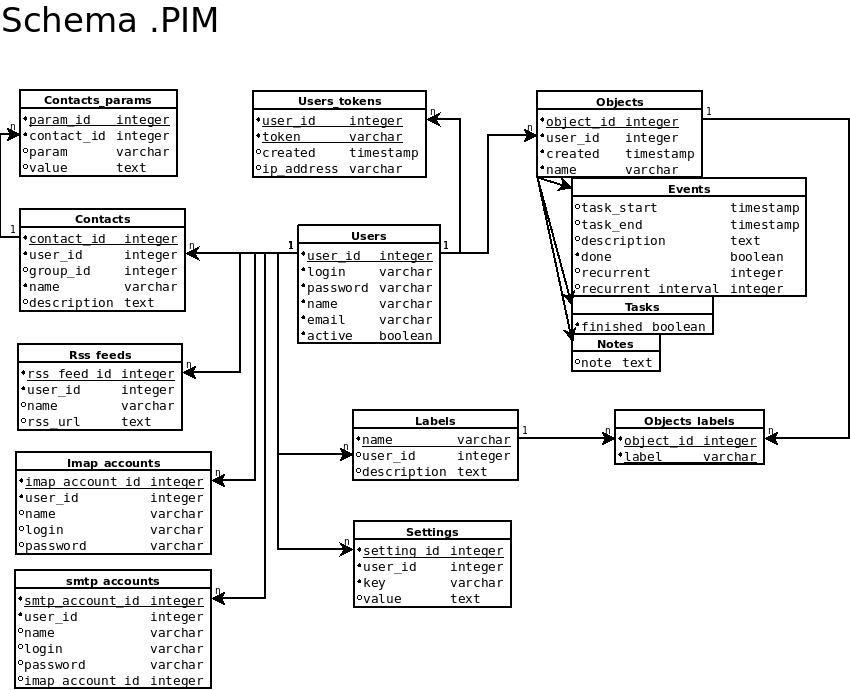
\includegraphics[width=\textwidth]{../structure.png} 
\newpage
Popis jednotlivých tabulek
\begin{itemize}
  \item Users - tabulka pro uživatele aplikace
    \begin{itemize}
      \item login - přihlašovací jméno
      \item password - MD5 hash přihlašovacího hesla
      \item name - jméno uživatele
      \item email - kontaktní email
      \item active - boolean příznak, jestli má uživatel povoleno přihlášení, nebo je blokovaný
    \end{itemize}

  \item Users\_tokens - tabulka pro trvalé přihlášení
    \begin{itemize}
      \item user\_id - uživatel
      \item token - vygenerovaný 32 znakový token
      \item created - datum vytvoření - tokeny starší 90 dní už nejsou platné
      \item ip\_address - IP adresa, z~které byl token vytvořen
    \end{itemize}
    
  \item Contacts - tabulka kontaktů
    \begin{itemize}
      \item name - název kontaktu
      \item description - popis, nebo poznámka
    \end{itemize}

  \item Contacts\_params - jednotlivé položky kontaktu. Každý kontakt může mít libovolný počet položek, například email, telefon a~adresu
    \begin{itemize}
      \item contact\_id - cizí klíč s~vazbou na kontakty
      \item param - název položky - např. email nebo telefon
      \item value - konkrétní hodnota - např. konkrétní telefon nebo email
    \end{itemize}

  \item Rss\_feeds - nastavení RSS - jednotlivé účty a~jejich URL pro synchronizaci
    \begin{itemize}
      \item name - název, jen pro přehlednost a~výpis v~menu
      \item rss\_url - URL adresa XML feedu
    \end{itemize}

  \item Imap\_accounts - Účty IMAP klienta
    \begin{itemize}
      \item name - název účtu
      \item login - přihlašovací jméno
      \item password - heslo - v~plaintextu pro přihlášení k~IMAPu
      \item host - IMAP server
      \item port - IMAP port (výchozí 143)
      \item ssl - boolean příznak pro zabezpečené spojení SSL
    \end{itemize}

  \item Smtp\_accounts - Účty pro odchozí poštu
     \begin{itemize}
	\item name - název účtu
	\item login - přihlašovací jméno
	\item password - heslo - v~plaintextu pro přihlášení k~IMAPu
	\item host - SMTP server
	\item port - SMTP port (defaultně 25)
	\item ssl - boolean příznak pro zabezpečené spojení SSL
      \end{itemize}

  \item Objects - rodičovská tabulka ze které dědí Events, Tasks a~Notes
    \begin{itemize}
      \item object\_id - sdílený primární klíč, generuje se ze sekvence
      \item name - název objektu (Úkolu, události nebo poznámky)
    \end{itemize}

  \item Events - tabulka událostí v~kalendáři
      \begin{itemize}
	\item task\_start - datum začátku události
	\item task\_end - datum konce události
	\item description - textový popis
	\item done - boolean příznak, true pokud je událost již dokončena/splněna
	\item recurrence - boolean příznak opakování
	\item recurrence\_interval - interval opakování (počet dní)
      \end{itemize}
  
  \item Tasks - tabulka úkolů
      \begin{itemize}
	\item finished - boolean příznak, true pokud je úkol již splněn
      \end{itemize}
  \item Notes
      \begin{itemize}
	\item note - poznámka, využívá se i~jednoduchého HTML formátování (odrážky, číslování, styly textu)
      \end{itemize}
  \item Labels - štítky
      \begin{itemize}
	\item name - název štítku
	\item description - textový popis
      \end{itemize}
  \item Objects\_labels - vazební tabulka štítků na objekty
  \item Settings - tabulka pro jednotlivá nastavení uživatele
      \begin{itemize}
	\item key - název konstanty
	\item value - hodnota
      \end{itemize}
\end{itemize}

Dále jsou definovány procedury v~jazyce plpgsql, který PostgreSQL poskytuje. SQL procedury jsou spouštěny na SQL serveru, odpadá tedy režie přenosu dat a~také je mohou spouštět triggery. Trigger je definovaná činnost, která se má provést při databázové operaci nad tabulkou. Triggery mohou např. spouštět SQL procedury po INSERT, UPDATE nebo DELETE operaci.
V~PIM aplikaci se využívá trigger ke generování tokenů pro trvalé přihlášení, více v kapitole \ref{sec:authentization}. 
Tento trigger se spustí po vložení záznamu do users\_tokens a~vygeneruje 32 bitový náhodný řetězec.

Mezi další funcki patří plpgsql procedura pro přiřazování štítků k~objektům. Zajistí vytvoření nového štítku, pokud uvedený ještě neexistuje, v~opačném případě použije již existující.


\section{Implementace serverové aplikace}
\label{sec:ServerArchitecture}
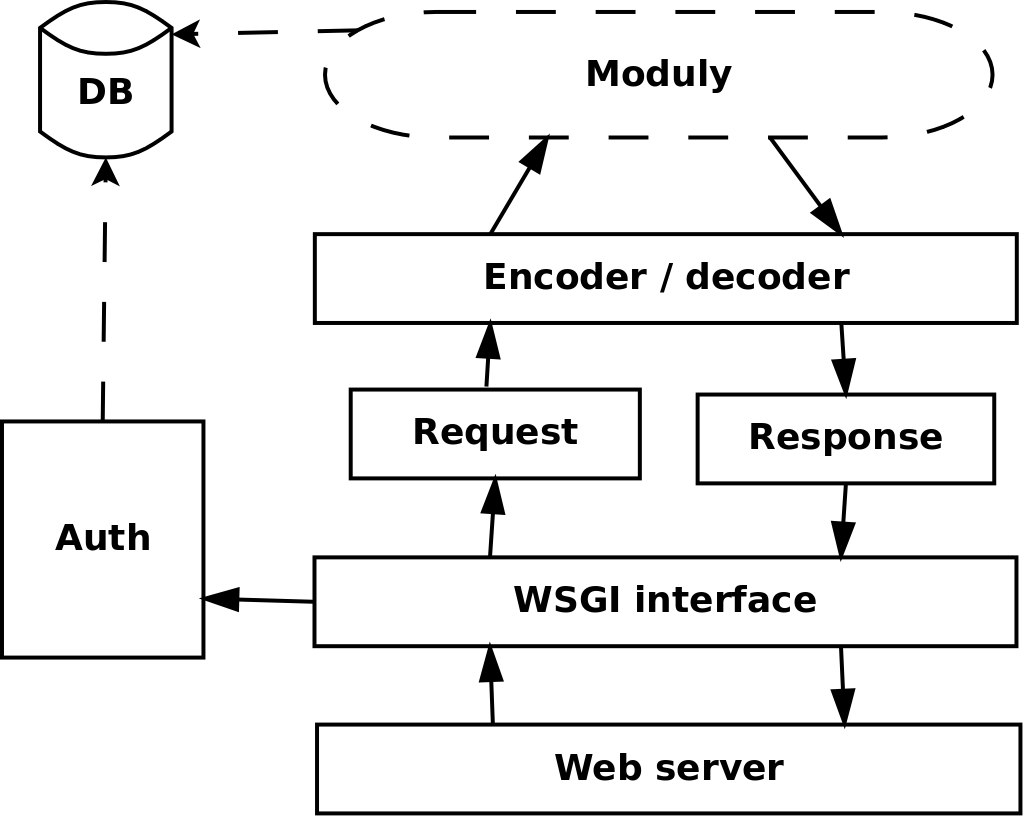
\includegraphics[scale=0.6,width=10cm,height=10cm]{../serverArchitecture.png} 
\bigskip

Serverová strana je napsaná ve skriptovacím jazyce Python,
pro spolupráci s~webovým serverem využívá WSGI rozhraní, což je nástupce mod\_python.
WSGI umožňuje, aby aplikace běžela po celou dobu běhu webového serveru a~každý příchozí požadavek byl zpracován v~jednom vlákně.
WSGI požaduje skript obsahující metodu application a~předává parametry environ a~start\_response.

Environ je objekt obsahující proměnné webového serveru, parametry HTTP požadavku a~mnoho dalšího.

``start\_response'' je metoda, která slouží k~zahájení odpovědi, předávají se dva parametry, z~nichž první je HTTP stavový kód a~druhý jsou HTTP hlavičky.

Zjednodušeně vstupní skript serveru může vypadat takto:
\bigskip
\begin{lstlisting}[label=src:Python,caption=Ukázka WSGI aplikace]

def application(environ, start_response):
	
	.... obslužný kód...
	
	start_response('200 OK', (
		['content-type', 'text/plain']
	))
\end{lstlisting}
Referenční implementace WSGI nijak nepřispívá ke zjednodušení zpracování HTTP požadavku, slouží jen jako mezivrstva HTTP serveru a~Python aplikace, pouze předá asociativní pole s~proměnnými HTTP serveru, kde se nachází jak tělo požadavku, tak konkrétní URL.
V~tomto serveru je WSGI skript použit pouze jako mezivrstva mezi webovým serverem a~vlastními třídami.
WSGI umožňuje tzv. middleware, což je obalení aplikace další vrstvou, v~PIM aplikaci se využívá knihovny beaker
a~middleware SessionMiddleware, která implementuje podporu session. Session dává HTTP serveru možnost uložit si
libovolné informace s~vazbou na konkrétního uživatele. Používá se především pro identifikaci přihlášeného uživatele a~pro zjištění jeho ID (odpovídá user\_id v~tabulce Users v~databázi)

Adresářová struktura serveru má konkrétní význam a~rozdělení
\begin{itemize}
\item auth - třídy sloužící k~autentizaci uživatelů - např. z~databáze nebo LDAP
\item config - konfigurační soubory
\item datasources - třídy zdrojů dat - např. PostgreSQL databáze, souborový systém
\item lib - obecné knihovny serveru
  \begin{itemize}
    \item encoders - vrstvy enkodéru/dekodéru pro serializaci objektů a~dat do JSON formátu
  \end{itemize}
\item modules - moduly poskytující konkrétní data a~operace nad určitými daty
 \begin{itemize}
    \item mail - IMAP a~SMTP klient
	\begin{itemize}
	    \item maillib - knihovna pro přístup k~IMAP a~SMPT
	\end{itemize}
    \item rss - RSS čtečka
    \item timetable - návrhář VŠB rozvrhu
  \end{itemize}
\item templates - HTML šablony pro přihlášení a~samotné web aplikace
\end{itemize}


\subsection{Zpracování HTTP požadavku}
% O zpracování HTTP požadavku se stará třída Request v knihovně lib.
% Při příchozím HTTP požadavku se vždy vytvoří nová instance této třídy, v konstruktoru se ji předá proměnná environ.
% Při vytvoření instance se rozparsuje environ, který obsahuje tělo POST i GET požedavku, ošetření vstupních polí,
% případně vložení do File objektu, pokud se jedná o soubor.
% 
% WSGI skript pak zavolá metodu dispatch(), která se postará o nalezení konkrétního modulu podle URL,
% při nenalezení se automaticky spouští notFound metoda z třídy errors.
% 
% Nalezený modul musí mít konstruktor přijímající jeden parametr - instanci session, pak se volá metoda určená v poslední části URL
% Moduly v URL lze libovolně zanořovat, poslední část vždy určuje volanou metodu.
% 
% Implementace modulu by měla splňovat interface definovaný v třídě lib.Module, každý modul může tuto třídu zdědit a metody implementovat
% Pro snažší implementaci může dědit lib.sqlModule, který usnadňuje SQL dotazy - více v sekci \ref{sec:ModuleInterface}
% 
% Po vrácení odpovědi(dat) od modulu se tato odpověď zabalí do objektu Response, který zajistí nastavení správných HTTP hlaviček,
% včetně serializaci dat do požadované podoby (JSON). Vzhledem k rozvrstvení implementace lze formát JSON jednoduše zaměnit za XML
% záměnou třídy provádějící serializaci



Jako základ zpracování HTTP požadavku slouží třída Request, které v~konstruktoru předáme
environ proměnnou, obsahující vše z~HTTP požadavku.
Hned při provádění konstruktoru se environ a~jeho proměnné rozparsují na interní proměnné get, která obsahuje proměnné z~URL (GET požadavek), post, která obsahuje tělo HTTP požadavku (metoda POST) a~request, která obsahuje obojí, přičemž při shodě názvu proměnných má přednost POST (POST přepíše GET).

Při příchodu požadavku můžeme také nastavit encoder, tedy jaká knihovna bude použita pro serializaci dat, jako výchozí se používá JSON.

Po vytvoření instance třídy lib.Request se volá metoda dispatch(), která zajišťuje zavolání konkrétního modulu,
serializaci dat a~vrácení instanci třídy Response.

Třída lib.Response obaluje HTTP odpověď, nastavuje správné HTTP hlavičky a~stavové kódy.
WSGI při vracení odpovědi přijímá iterátor, třída request rozhraní iterátoru implementuje, takže lze využít streamování dat po předem nastavené velikosti bloku dat. To vede ke zmenšení zátěže serveru a~snížení využité paměti, protože pokud se streamuje velký datový objekt, díky rozhraní iterátoru nemusí být načten v~paměti celý, ale pouze předem nastavená velikost bloku.

Environ obsahuje položku "PATH\_INFO", která obsahuje část URL za adresou serveru. Tuto část URL rozdělíme podle lomítek, a~určíme tak jméno konkrétního modulu.
Poslední část URL určuje název metody v~modulu.

Pokud k~dané URL byl nalezen modul, včetně spouštěné metody, předáme metodě parametry z~HTTP požadavku, ale pouze ty, které daná metoda vyžaduje.
K~tomu slouží knihovna "inspect", konkrétně "inspect.getargspec". Tím je ošetřeno, že metoda dostane pouze ty parametry, které má uvedené ve své definici.


\subsection{Autentizace}
\label{sec:authentization}
K~jakékoliv interakci se serverem musí být uživatel přihlášen, v~opačném případě server vrátí přihlašovací formulář z~templates/login.html.

Informace o~přihlášeném uživateli včetně jeho user\_id se ukládá do session, pokud v~session není, automaticky se pokládá za nepřihlášeného. 
Pro pohodlnost a~usnadnění použití může být přihlášení trvalé - od uživatele tedy nebude vyžadováno žádné jméno ani heslo.
Trvalé přihlášení funguje na principu ukládání speciálních vygenerovaných tokenů, což jsou náhodné řetězce o~délce 32 znaků.
Tokeny se ukládají do cookies na straně klienta a~do databáze na straně serveru. Cookie je malé úložiště dat v~internetovém prohlížeči a~tyto data jsou odesílány na server s~každým požadavkem. Tímto způsobem se tedy uloží do databáze vygenerovaný token spolu s~uživatelským ID a~zároveň se odešle ke klientovi. Data, která jsou uložena v~cookies, mohou mít nastavenou dobu platnosti. V~tomto případě je nastavena platnost na 90 dní. Při příštím spuštění aplikace internetový prohlížeč automaticky odešle na server uložený token, v~databázi se ověřuje, kterému konkrétnímu uživateli token patří, ten pak bude považován za přihlášeného.
Délka tokenu byla zvolena na 32 znaků z~důvodu bezpečnosti - čím delší token, tím složitější je uhádnout token a~vydávat se za jiného uživatele.
Tokenů lze vygenerovat pro jednoho uživatele více, aby bylo možné využívat trvalé přihlášení z~více míst nebo z~více prohlížečů.

U~nepřihlášeného uživatele server.wsgi vždy pro zpracování HTTP požadavku využívá třídu AuthRequest, která vrací přihlašovací formulář a~při odeslání přihlašovacích údajů je ověří pomocí objektu Auth.

Třída Auth implementuje validační funkci "authenticate" přijímající dva parametry - login a~heslo, která provádí ověření uživatele v~databázi, případně může využívat jiné autentizační mechanismy (např. LDAP, unix PAM atd...). 

Metoda authenticate vrací asociativní pole s~uživatelským ID a~jeho rolí v~systému - buďto admin, nebo "user" - což je obyčejný uživatel.
Admin má práva přidávat a~spravovat další uživatele.

Vzhledem k~tomu, že PIM aplikace není předurčena pro široké použití na veřejných serverech, ale spíše na privátních pro pár uživatelů, není povolena registrace, ale uživatele může vytvářet jen administrátor.



\newpage
\subsection{Datové typy, validace dat}
\label{sec:dataTypes}
V~komunikačním protokolu a~jeho popisech datových sloupců se uvádí povinný atribut "type", což značí datový typ. Datové typy jsou předem definované třídy, které implementují validaci a~případně transformaci příchozích dat pro uložení do databáze.

Datové typy jsou deklarovány v~lib.dataTypes a~povětšinou implementují rozhraní IType.
V~Pythonu se rozhraní chová stejně jako třída, je to tedy jen "konvence" pro programátora, nikoliv striktní požadavek na implementaci.

\bigskip
\begin{lstlisting}[label=src:Python,caption=Rozhraní datového typu]
class IType(object):

	def __init__(self):
		raise Exception("Not implemented yet")

	def validate(self, value):
		raise Exception("Not implemented yet")

	def __str__(self):
		raise Exception("Not implemented yet")

	def encode(self, value):
		return value

	def decode(self, value):
		return value
                
\end{lstlisting}

\begin{itemize}
\item \_\_init\_\_, přesněji konstruktor, slouží jen k~vlastní inicializaci datového typu. Může přijímat libovolný počet parametrů, které se mu předají při vytváření instance ve specifikaci modulu
\item validate je metoda pro ověření správnosti dat, přijímá pouze jednu konkrétní hodnotu v~parametru a~vrací True nebo False. Samotný kód metody může data ověřovat libovolným způsobem, nejčastěji se využívá knihovny \uv{re} pro ověření regulárním výrazem, nebo jen např. omezení rozsahu čísla (integer)
\item \_\_str\_\_ vrací pouze název datového typu jako řetězec, tedy jak se bude datový typ jmenovat ve specifikaci sloupce v~komunikačním protokolu.
\item encode ošetřuje příchozí data při ukládání do databáze, nejčastěji se escapují určité sekvence textového řetězce
\item decode je inverzní funkce k~encode - dekóduje data uložena v~databázi při odesílání ke klientovi
\end{itemize}


Vzhledem k~objektovému návrhu datových typů se nové typy dají snadno zdědit z~již existujících. Výhodné je to tehdy, pokud chceme například jen informovat klienta, že má použít jiný prvek (widget) k~editaci.
Toho se využívá např. u~datového typu HTML, což je v~podstatě textový řetězec, ale pro editaci se používá HTML editor.

\bigskip
\begin{lstlisting}[label=src:Python,caption=Ukázka implementace datového typu]
class String(IType):
	regexp = None
	def __init__(self, regexp = None):
		self.regexp = regexp

	def validate(self, value):
		if not self.regexp:
			return True

		return False

	def __str__(self):
		return 'String'

\end{lstlisting}

\begin{lstlisting}[label=src:Python,caption=Dědičnost datového typu]
class HTML(String):
	def __str__(self):
		return 'HTML'
\end{lstlisting}
                

\newpage
\subsection{Automatizované SQL dotazy, transakce}
\label{sec:sql}
Vzhledem k~tomu, že je aplikace založená převážně na SQL databázi, je vhodné manipulaci s~databázi co nejvíce zjednodušit. Vše se nachází v~knihovně lib.sqlReport, která obsahuje třídy pro SELECT, INSERT, UPDATE a~DELETE.

Při práci s~databází všem třídám (pro jakoukoliv operaci) předáváme definice sloupců.
Definice sloupců je instance třídy Column, která obsahuje veškerý popis dat ukládaných ve sloupci, stejně jako se přenáší ke klientovi komunikačním protokolem.
Konstruktor této třídy má jediný parametr - asociativní posle s~parametry.

\begin{itemize}
\item name - název sloupce, bude se zobrazovat na klientské straně
\item id - identifikátor, který určuje přesný název sloupce výsledného dotazu, tedy název sloupce, případně název aliasu pokud byl v~dotazu použit
\item visibility - pole, které určuje viditelnost na klientské aplikaci
	\begin{itemize}
		\item static - viditelné při zobrazování dat
		\item edit - viditelné při editaci
	\end{itemize}
	nebo prázné pole - tedy nebude viditelné nikdy.
\item required - restrikce, jestli je hodnota vyžadována při editaci, tedy je povinná
\item insertable - boolean příznak, jestli lze data tohoto sloupce vkládat (INSERT) do databáze. Např. primární klíč, který je generován přímo databází má nastaveno false.
\item editable - boolean příznak obdobně jako insertable, značí jestli je sloupec upravit pomocí UPDATE
\item flags - pole s~přídavnými informacemi, např. "primaryKey", jestli je sloupec primárním klíčem v~databázi
\item default - výchozí hodnota sloupce - pokud SQL dotaz vrátí NULL, použije se tato hodnota
\item type - instance třídy datového typu, více \ref{sec:dataTypes}
\item searchAlias - šablona pro WHERE podmínku. Pokud např. hledáme určitou shodu řetězce pomocí LIKE operátoru, do searchAlias můžeme napsat výraz, kde \%s bude nahrazeno konkrétní hodnotou
\item value - pevně daná hodnota sloupce
\end{itemize}

Všechny třídy pro práci s~databází dědí ze třídy ColumnParser, která zjednodušuje práci s~definicemi sloupců, validaci dat a obsahuje další podpůrné funkce.

\subsubsection{SQLReport}

Třída SQLReport slouží pro získávání dat z~databáze (operace SELECT). Při vytváření instance se v~konstruktoru předává zformátovaný řetězec konkrétního SQL dotazu. V~SQL dotazu se nesmí uvádět klauzule WHERE, ORDER a~LIMIT/OFFSET. Místo těchto klauzulí se zapisují zástupné konstanty. Tyto zástupné konstanty se pak převedou na automaticky vygenerovaný SQL kód. Konstanty se zapisují ve formátu \uv{\%(nazev)s}, je to nativní zápis formátování v~jazyce Python.

Dostupné konstanty:
\begin{itemize}
 \item where - místo, kam se má vložit podmínka, která se nastavuje metodou setFilter, případně setFixedFilter
 \item order - místo, kam se vloží názvy sloupců řazení
 \item limit - místo, kam se vloží omezení počtu výsledných záznamů, včetně offsetu
\end{itemize}

Po vytvoření instance třídy SQLReport je nutné předat definice sloupců pomocí metody setColumns.
Po předání definice sloupců lze libovolně nastavovat podmínky. K~tomu slouží metody setFixedFilter a~setFilter.
Podmínky předané pomocí setFixedFilter zaručují vynucené použití v~každém dotazu a~možnost obsáhnout v~podmínce i~sloupce, které nebyly předem definované. Toho se využívá převážně k~vazbě dat na uživatele, jehož ID je v~session.
Třída SQLReport dále obsahuje metodu setOrder pro řazení výsledků, které se v~parametru předává asociativní pole, kde klíče v~poli jsou názvy sloupců a~hodnoty nabývají \uv{ASC} pro vzestupné, případně \uv{DESC} pro sestupné řazení.
SQLReport ještě umožňuje omezení počtu výsledků a~to metodou setLimit se dvěma argumenty, první pro počáteční pozici v~datech a~druhý parametr určuje celkový počet výsledků.
\bigskip
\begin{lstlisting}[label=src:Python,caption=Ukázka použití třídy SQLReport]
def getData(self, query):
	result = SQLReport("SELECT * FROM pim.events %(where)s %(order)s %(limit)s")
	result.setColumns(self.columns)
	result.setFixedFilter("user_id = '%s'" % self.session['user_id']) 
	result.setFilter(query)
	return result.getReport()
\end{lstlisting}
\newpage
\subsubsection{SQLUpdate}
Třída SQLUpdate poskytuje jednoduché rozhraní pro aktualizaci záznamů v~databázi. Všechny třídy z~knihovny lib.sqlReport se chovají obdobně. Konstruktor SQLUpdate přebírá název tabulky, která se má aktualizovat.
Vzhledem k~tomu, že UPDATE v~SQL databázích vypadá často podobně, stačí jen pomocí metody setKey nastavit WHERE podmínku. Metoda setKey se chová stejně jako setFilter u~SQLReport. Nakonec se objektu předají data ve formě asociativního pole metodou setData.
\bigskip
\begin{lstlisting}[label=src:Python,caption=Ukázka použití třídy SQLUpdate]
def update(self, key, data):
	result = SQLUpdate("pim.events")
	result.setColumns(self.columns)
	result.setKey({
		"event_id": 123
	})
	result.setData(data)
	
	return result.update()
\end{lstlisting}

\subsubsection{SQLInsert}
Třída SQLInsert zprostředkovává vkládání do databáze. Chování má identické jako třída SQLUpdate, jen se nenastavuje podmínka, která je u~operace INSERT zbytečná. Funkce spouštějící SQL dotaz, tedy insert(), vrací primární klíč vloženého záznamu, pokud byl v~definicích sloupců uveden.

\bigskip
\begin{lstlisting}[label=src:Python,caption=Ukázka použití třídy SQLInsert]
result = SQLInsert("pim.events")
result.setColumns(self.columns)
result.setData(data)
result.setAdditionalData({
	'user_id': self.session['user_id']
})
result.insert()

\end{lstlisting}

\subsubsection{SQLDelete}
Poslední třídou, kterou knihovna sqlReport disponuje, je SQLDelete sloužící k~mazání záznamů z~databáze.
Chování má taky obdobné jako třída SQLUpdate, s~tím rozdílem, že se nenastavují data, ale pouze podmínka, podle které se řádky odstraňují.
Při používání SQLDelete je nutné podmínku uvést, protože PostgreSQL by bez uvedení podmínky smazal všechny záznamy. Z~tohoto důvodu třída SQLDelete záměrně nepodporuje mazání bez podmínky, protože se to v~PIM nikde nevyužívá (přinejmenším bývá vždy vazba podmínky na ID uživatele).

\bigskip
\begin{lstlisting}[label=src:Python,caption=Ukázka použití třídy SQLDelete]
result = SQLDelete("pim.events")
result.setColumns(self.columns)
result.setFilter({
	'event_id': 123
})

result.delete()
\end{lstlisting}

\subsubsection{SQL rozhraní}
Pro připojení k~PostgreSQL se na serveru vytváří pool, tedy objekt, který obsahuje blíže nespecifikované množství trvalých připojení k~databázi a~tyto připojení se z~poolu vybírají a~vrací.
Při práci s~databází je z~poolu vyžádán objekt připojení, ten se z~poolu vyjme po dobu, co se s~ním pracuje, pak se do poolu vrátí.
Přístup předem vytvořených spojení v~poolu má výhodu ve zmenšení režie neustálého připojování a~odpojování k~databázovému serveru.
Každé připojení vyjmuté z~poolu se do poolu zase musí vrátit, jinak by vznikl tzv. connection leak, v~poolu by objekty připojení došly a~aplikace by zhavarovala na nedostatek připojení.

Pool je definován v~knihovně datasources.postgres, konkrétně třída ConnectionPool. Tato třída implementuje kromě konstruktoru 3 metody. 
\begin{itemize}
 \item getconn - získává objekt připojení z~poolu
 \item putconn(objekt připojení) - vrací připojení zpět do poolu 
 \item query(sql dotaz) - jednoduché vykonání SQL dotazu, funkce obstará získání připojení, vykonání dotazu a~následné vrácení připojení do poolu
\end{itemize}

Získaný objekt připojení poskytuje metodu cursor(), která vytváří kurzor pro vykonávání SQL dotazů.
Kurzor je objekt, který umožňuje vykonání SQL kódu z Pythonu a existuje po celou dobu připojení k databázi.
Kurzor vytvořený ve stejném objektu připojení není izolovaný, tedy změny jednoho kurzoru uvidí jiný kurzor stejného objektu, i~když nebyl proveden commit


\subsubsection{Transakce}
Transakce je uspořádaná skupina databázových operací (dotazů, procedur), která se vnímá a~provádí jako jediná jednotka a~to celá, nebo vůbec ne. Nikdy nesmí nastat případ, kdy se vykoná jen její část. Transakce je vhodné používat při změnách ve více tabulkách, případně řetězení SQL operací. Tyto operace se tak provedou buďto všechny, nebo žádná.

Třída pro vykonávání transakcí SQLTransaction je implementována ve stejné knihovně jako pool připojení, tedy v~datasources.postgres.
Transakce se provádí tak, že se vytvoří instance této třídy, která poskytuje kurzor. S~tímto kurzorem se vykonávají SQL dotazy, při úspěšném provedení všech dotazů se spustí metoda commit() a~změny se trvale uloží do databáze.

Třídy pro práci s~databází, konkrétně SQLUpdate, SQLInsert, SQLDelete mohou přebírat v~konstruktoru instanci SQL transakce.
Tímto tyto třídy použijí pro své SQL dotazy stejný objekt připojení. Pak se v~kódu pomocí výjimek provede commit, který změny uloží nebo rollback, který vrátí změny do stavu před započetím transakce.


\begin{lstlisting}[label=src:Python,caption=Ukázka použití transakcí]
transaction = datasources.postgres.SQLTransaction()

try:
	a = SQLDelete("pim.events", transaction)
	...
	b = SQLUpdate("pim.events", transaction)
	...
	b = SQLInsert("pim.events", transaction)
	
	transaction.commit()
	
except Exception as e:
	transaction.rollback()
	
finally:
	transaction.close()

\end{lstlisting}
\newpage

\subsection{Moduly, rozhraní modulů}
\label{sec:modules}

Moduly, které mají poskytovat data klientovi, by měly implementovat specifické rozhraní a~vracet data ve sjednoceném formátu popsaném v~kapitole \ref{sec:communication}.
Rozhraní je definováno v~knihovně lib.Module, kterou lze zdědit nebo implementovat znovu. Pro rychlost a~jednoduchost psaní nových modulů, lib.Module implementuje základní operace s~databázemi, které jsou natolik automatizované, že stačí jen definovat sloupce a~databázovou tabulku. Z~těchto definic se vygenerují patřičné operace SELECT, INSERT, UPDATE a~DELETE. Pokud generované operace nejsou vyhovující, lze vždy danou metodu předefinovat.

\begin{itemize}
 \item \_\_init\_\_(session) - konstruktor, přijímá pouze objekt session, který obsahuje uložené data mezi jednotlivými HTTP požadavky
 \item getData(query, limit, offset) - metoda, která vrací konkrétní data. Objekt query slouží k~vyhledávání, limit a~offset ke stránkování dat
 \item getColumns - metoda bez parametrů, která vrací pouze specifikaci sloupců, více v~kapitole \ref{sec:sql}
 \item update(key, data) - metoda pro aktualizaci dat. Objekt key určuje konkrétní podmínku, které řádky se mají aktualizovat. Data obsahují nové hodnoty
 \item insert(data) - metoda pro vkládání dat
 \item delete(key) - metoda pro mazání dat. Objekt key obsahuje podmínku, které řádky se mají smazat
\end{itemize}

Třída lib.Module vyžaduje, aby byly v~třídní proměnné \uv{columns} definovány sloupce. Definice sloupců jsou instance třídy lib.sqlReport.Column v~poli. Dále také požaduje třídní proměnnou \uv{table}, která specifikuje tabulku, se kterou se bude pracovat.
Automaticky vygenerované SQL dotazy vždy ošetřují příchozí data a~kontrolují jejich správnost podle datových typů.

Při předefinování metod lze vykonat více SQL operací a~především je vhodné všechny tyto operace provádět v~transakcích.


\subsection{Modul RSS čtečky}
\label{sec:rss-server}
Součástí PIM aplikace je základní implementace RSS čtečky. V~databázi k~tomuto účelu existuje tabulka rss\_feeds, kde má každý uživatel uložené URL k~jednotlivým RSS feedům.

Modul je rozčleněn na 3 třídy:
\begin{itemize}
 \item Feed - výpis všech záznamů z~konkrétní URL
 \item FeedList - seznam dostupných RSS feedů
 \item rssSettings - administrace RSS feedů
\end{itemize}

K~samotnému parsování RSS feedu je využívána Python knihovna feedparser. Ta poskytuje třídu feedparser.parse, která vrací objekt s~RSS položkami v~atributu \uv{entries}. Ty se pak pouze zformátují tak, aby odpovídaly specifikacím sloupců a~odešlou na klienta k~zobrazení.



\subsection{Modul E-Mailového klienta}
\label{sec:mailClient}
Základem pro emailový klient je využití vestavěné knihovny imaplib a~smtplib v~Pythonu. Imaplib poskytuje nízkoúrovňové rozhraní pro IMAP účty, práce s~tímto rozhraním je těžkopádná a~nepohodlná. To vedlo k~implementaci vrstvy využívající imaplib a~implementaci funkcí usnadňující tvorbu modulu.

\bigskip

Modul emailového klienta je rozdělen na tyto části:
\begin{itemize}
 \item folderTree - pouze vrací strom složek
 \item imapSettings - poskytuje IMAP nastavení
 \item smtpSettings - poskytuje SMTP nastavení
 \item mailList - vrací seznam emailů konkrétní složky
 \item mailMessage - vrací tělo emailu a~umožňuje odeslat nový email
\end{itemize}

IMAP (Internet Message Access Protocol) je internetový protokol pro vzdálený přístup k~e-mailové schránce. Na rozdíl od protokolu POP3 umí IMAP pracovat v~tzv. on-line i~off-line režimu a~nabízí pokročilé možnosti vzdálené správy (práce se složkami, přesouvání zpráv, prohledávání na straně serveru a~podobně). V~současné době se používá protokol IMAP4 (IMAP version 4 revision 1 - IMAP4rev1), který je definován v~RFC 3501.
\cite{imap-wiki}

Vrstva pro IMAP obsahuje pouze jednu třídu maillib.Imap. Ta v~konstruktoru přebírá ID uživatele a~ID účtu, ke kterému se má připojit.
Všechny IMAP účty včetně nastavení jsou uloženy v~databázové tabulce imap\_accounts. ID uživatele IMAP vrstva přebírá pouze pro kontrolu, jestli konrétní účet tomuto uživateli náleží. Předejde se tak útoku, kdy by uživatel zkoušel v~požadavku uvádět cizí ID.
IMAP vrstva si vytvoří instanci IMAP4 objektu z~imaplib, případně IMAP4\_SSL, pokud jde o~zabezpečené spojení.

Vrstva poskytuje především konverzi IMAP struktur do vlastních formátů, například parsování adresářové struktury do stromu a~převod datumu na nativní objekty jazyka Python. 
Dále tato třída poskytuje metody:

\begin{itemize}
 \item login(login, password) - přihlášení uživatele
 \item getFolderTree - vrátí adresářový strom v~asociativním poli
 \item getMailList(directory, searchParams) - vrátí seznam emailů konkrétní složky (výchozí je \uv{INBOX})
 \item getMail(mailId, folder) - vrátí tělo konkrétního emailu. Je nutné předat i~název složky
 \item close - korektní ukončení spojení
\end{itemize}


\bigskip

Pro odesílání se využívá vestavěné knihovny smtplib. Její použití je snadnější a~jednodušší než imaplib, takže bylo zbytečné vytvářet další vrstvu. V~modulu se vytvoří spojení na SMTP server včetně přihlášení, přidá se emailová zpráva v~podobě MIME a~odešle.

MIME, plným názvem Multipurpose Internet Mail Extensions („Víceúčelová rozšíření internetové pošty“), je internetový standard, který umožňuje pomocí elektronické pošty zasílat zprávy obsahující text s~diakritikou, lze k~ní přiložit přílohu v~nejrůznějších formátech, umožňuje funkci digitálního podpisu apod. V~současné době ho využívají i~další protokoly aplikace (např. HTTP). Standard MIME je definován šesti dokumenty: RFC 2045, RFC 2046, RFC 2047, RFC 4288, RFC 4289 a~RFC 2049.
\cite{smtp-wiki}

Samotná zpráva je pak včetně HTML formátování zabalena ve třídě MIMEText s~kódováním UTF-8.




% \label{sec:architektura-server}

\section{Implementace klientské aplikace}
Aby byla klientská aplikace multiplatformní a~dostupná kdekoliv, využívá se RIA architektury v~internetovém prohlížeči.
Celá klientská aplikace funguje na principu načtení počáteční prázdné stránky bez jakýchkoliv elementů a~následné vykreslování (renderování) jednotlivých GUI prvků pomocí programovacího jazyku JavaScript. V~dnešní době je rychlost JavaScriptu více než dostačující, využívá se mnoho optimalizací včetně JIT compileru.

Aplikace vykreslí kompletní GUI pomocí vlastních prvků a~veškeré data odesílá i~stahuje komunikačním protokolem pomocí AJAX požadavku. AJAX je asynchronní požadavek na server, který běží na~pozadí a~při odezvě vyvolá předem definovanou událost.
Veškerá interakce s~uživatele využívá AJAX požadavků a~překreslení pouze určité oblasti aplikace, stránka se tedy nikdy nepřekresluje celá, tímto se docílí téměř okamžité odezvy bez problikávání obdobně jako v~nativních aplikacích.

\bigskip
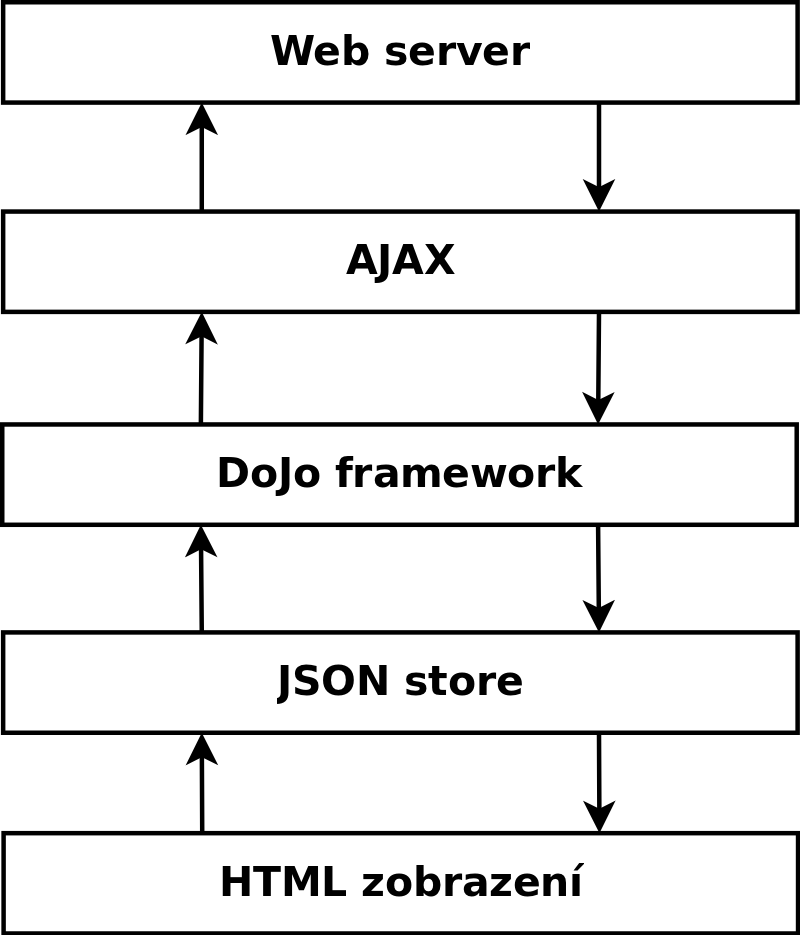
\includegraphics[width=0.4\textwidth]{../clientArchitecture.png} 


\subsection{DoJo - objektový JavaScript}
Vykreslování jednotlivých GUI komponent a~widgetů usnadňuje použitý framework DoJo, který do JavaScriptu zavádí objektivně orientované programování, včetně dědičnosti tříd a~funkce pro práci s~objekty.

DoJo obsahuje nebo je rozděleno na 3 části. Základní část je nedělitelná, často označována jako \uv{core} obsahuje funkci pro práci s~DOM objektem. DOM objekt je strom rozparsované HTML stránky, tedy rozhraní mezi HTML strukturou a~JavaScriptem. Jakákoliv změna v~DOM stromu se ihned projeví v~HTML struktuře a~naopak. Základní část DoJo toolkitu taktéž obsahuje podpůrné součásti pro objektově orientované programování, deklaraci tříd a~dědičnosti, včetně ostatních nástrojů např. pro AJAX požadavky na server, snadné CSS stylování HTML prvků a~mnoho dalšího.

Druhou částí je knihovna Dijit, která staví na objektovém programování a~vytváří snadno použitelné GUI prvky, kontejnery pro tvorbu GUI, ovládací a~vstupní widgety. 

Třetí částí je knihovna DojoX, označována jako DoJo Experimental, kde se nachází experimentální, nové, případně neotestované části jak GUI prvků, tak samotných funkcí DoJo. Z~DojoX se jednotlivé části přesunují do \uv{core} nebo dijit po otestování a~prohlášení za stabilní. 


\subsubsection{GUI prvky}
\label{sec:dojo-gui}
Veškeré GUI prvky dědí ze základní třídy dijit.\_Widget. Tato třída implementuje základní strukturu GUI prvku tak, jak ji vyžaduje DoJo.
Základní, kořenový HTML prvek, se nachází v~třídní proměnné domNode. Tento HTML prvek může obsahovat libovolnou HTML strukturu, ale ve frameworku se pracuje pouze s~celou třídou, do HTML prvků by se zasahovat nemělo.

dijit.Widget implementuje základní události, které můžeme přepsat, nebo využít návrhového vzoru observer a~na tyto události se napojit.
\bigskip
Životní cyklus DoJo widgetu:
\begin{itemize}
  \item constructor - konstruktor objektu
  \item postMixInProperties - metoda, která volána před samotným započetím vykreslování, tady lze ovlivnit všechny počáteční proměnné objektu
  \item buildRendering - pokud je zděděn i~předek dijit.\_Templated, zde se parsuje HTML šablona do DOM stromu
  \item postCreate - typicky metoda pro vykonání vlastního kódu po vytvoření prvku
  \item startup - metoda, která je volána po vložení prvku do DOM stromu, tedy do HTML stránky
  \item destroy - destruktor, v~této metodě by se měly odstranit veškeré interní objekty a~instance pro garbage collector
\end{itemize}

\begin{lstlisting}[label=src:JavaScript,caption=Třídy v~DoJo toolkit]
dojo.declare("myObject", dijit._Widget, {
	constructor: function(args) {
		this.param1 = args.param1;
		this.param2 = args.param2;
		
		this.inherited(arguments);
	},
	
	onClick: function(event) {
		console.log("clicked", event);
	}
})
\end{lstlisting}

Při vytváření tříd pomocí DoJo je vhodné dbát na předem určenou štábní kulturu. Především při vytváření instance se parametry vždy předávají jako asociativní pole (v~JavaScriptu a~dále jako objekt). Tímto objektem lze při vytváření instance přepisovat i~jednotlivé metody.

\bigskip
\begin{lstlisting}[label=src:JavaScript,caption=Třídy v~DoJo toolkit]
	var instance = new myObject({
		name: "nazev",
		onClick: dojo.hitch(this, function(event) {
			this.onMouseClick(event);
		})
	});
\end{lstlisting}

Vzhledem ke koncepci JavaScriptu je kontext volané funkce vždy kontext původní, tedy nepřepsané funkce. Pokud třída \uv{myObject} definuje funkci onClick, a~v~konstruktoru je přepsána jinou funkcí, kontext (třídní proměnná this) je třída myObject, nikoliv třída ve které je instance vytvořena a~funkce přepsána. Předejít této situaci se dá pomoci funkce dojo.hitch, která obalí funkci do správného kontextu, v~tomto případě třídy ve které vytváříme instanci, nebo pomocí uzávěrů, což se ale příliš nedoporučuje z~důvodu možných vzniků memory leaků (úniku paměti).



\subsection{Architektura a~design aplikace}
V~klientské aplikaci se využívá především zobrazovacích prvků z~knihovny Dijit, případně dědění ze základních tříd a~implementace vlastních prvků.

Aplikace se dělí na dvě hlavní části - GUI a~Widgety. Widgety implementují jednotlivé zobrazovací, případně vstupní prvky a~GUI pouze zobrazuje tyto prvky na obrazovce, případně umisťuje do konkrétních kontejnerů. Tomu odpovídá i~adresářová struktura aplikace:

\begin{itemize}
 \item app
    \begin{itemize}
     \item config - statické konfigurační soubory
        \begin{itemize}
	    \item Dashboard.js - dostupné widgety pro hlavní obrazovku
	    \item SiteMap.js - konfigurace jednotlivých pohledů a~menu
	\end{itemize}
     \item gui - implementace GUI
	\begin{itemize}
	 \item init.js - inicializace a~spouštění aplikace
	 \item Page.js - implementace zobrazené stránky (menu, kontejnery, vykreslování)
	\end{itemize}
     \item widgets - vlastní zobrazovací a~vstupní widgety
     \item templates - šablony pro DataForm, více v~kapitole \ref{sec:DataForm}
     
    \end{itemize}

\end{itemize}

Inicializace aplikace se provádí ve scriptu app/init.js, který vytváří instanci třídy app.gui.Page, tedy hlavní stránky, a~napojuje se na základní události jako je hashChange a~document.onkeypress. Událost hashChange je vyvolána při změně URL za znakem ``\#'', která se mění při změně sekce v~menu - tím se může přímo pomocí URL určit obsah k~zobrazení, takže lze odkazem otevřít podstránku i~v~JavaScriptu. Document.onkeypress je událost vyvolaná po stisku klávesy, takže lze využívat předem definované klávesové zkratky.

Dále se při inicializaci vkládá instance Page.js do DOM stromu, tím se zobrazí na stránce a~zavolá startup(), která se volá na každý widget po vložení do DOM stromu.

Vzhledem k~možnostem JavaScriptu init.js rozšiřuje některé nativní objekty, jako je String a~Date pro snadnější práci s~datem.

\bigskip
Základní koncept uživatelského rozhraní:

% 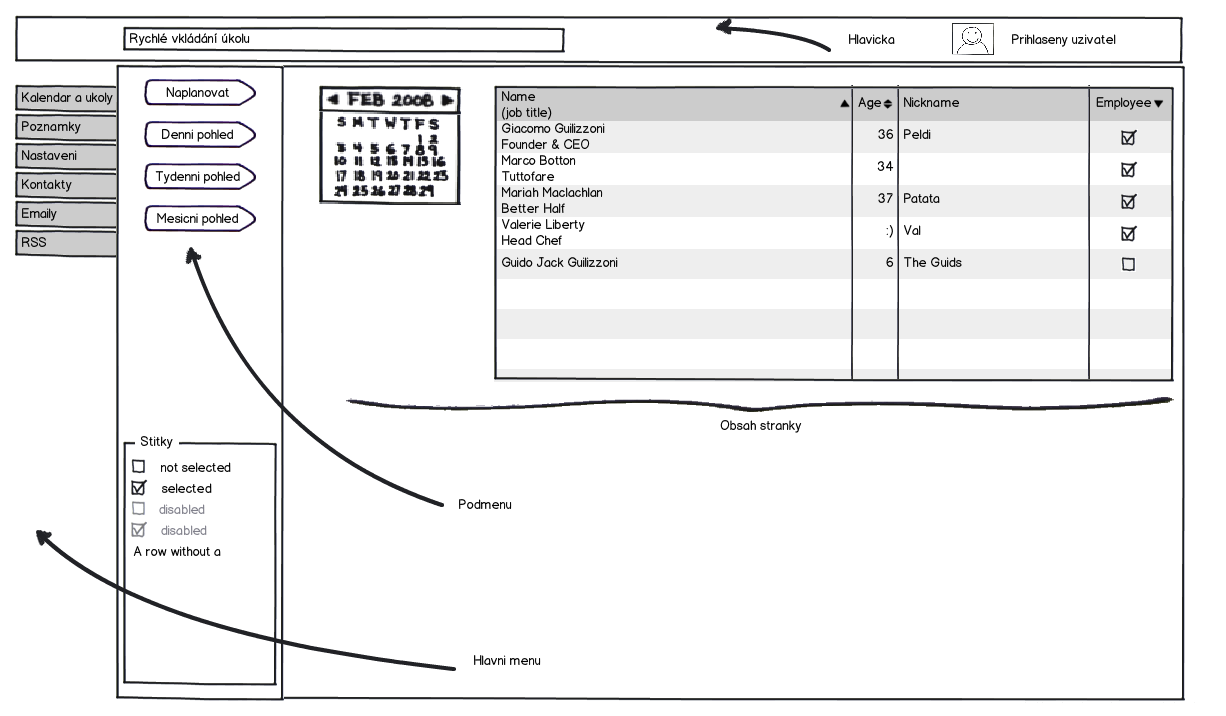
\includegraphics[width=\textwidth]{../guiConcept.png} 
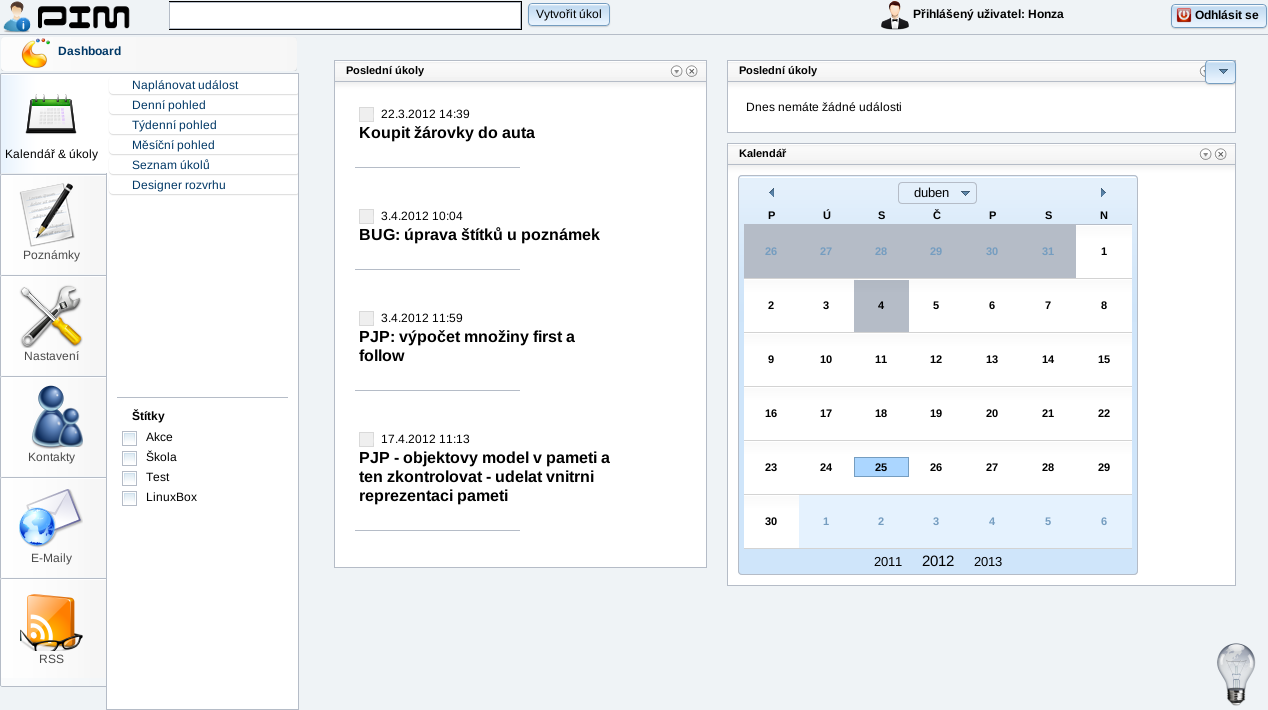
\includegraphics[width=\textwidth]{../screens/screen1.png} 

\subsubsection{Vykreslování stránek}
Třída app.gui.Page vytváří základní strukturu stránky - což je hlavička, kde se zobrazuje panel o~přihlášeném uživateli, levé menu a~kontejner pro vykreslování obsahu jednotlivých pohledů. Po celou dobu běhu aplikace se app.gui.Page nemění, pouze se překresluje kontejner s~pohledem konkrétní sekce.

Překreslování obsahu obsluhuje metoda onHashChanged, která je napojena na nativní událost prohlížeče hashChange reagující na změnu URL. Metoda nejprve odstraní původní obsah, zajistí korektní odstranění původní instance a~vytvoří novou instanci odpovídajícího obsahu. Instance obsahu a~jejich vazba na URL je konfigurovatelná v~konfigurační souboru app.config.SiteMap, podle kterého se i~vykresluje menu.

\newpage
\begin{lstlisting}[label=src:JavaScript,caption=Struktura SiteMap,extendedchars=true]
app.config.SiteMap = {
	mails: {
		title: "E-Maily",
		order: 3,
		menuProvider: app.gui.mail.MenuProvider,
		items: {
			mailBrowser: {
				page: app.gui.mail.MailBrowser,
				title: "Prohlížení",
			},
			newMail: {
				page: app.gui.mail.NewMail,
				title: "Napsat E-Mail",
			},
		}
	},
}
\end{lstlisting}

SiteMap konfigurace je JavaScriptový objekt a~jeho položky se větví do stromu. První úrověň vytváří kategorii v~menu a~druhou úroveň, tedy položky v~kategorii vytváří položka ``items``. Klíč názvu objektu je unikátní identifikátor, který se používá i~v~URL.
Položky v~kategorii se vykreslují automaticky dle konfigurace, nebo lze definovat vlastní widget uvedený v~menuProvider. Tento widget se vykreslí v~kategorii místo ostatních položek (na konfiguraci položek se pak nebere ohled).

Po překreslení obsahu se na instanci podstránky dále volá metoda onHashChanged, aby změna URL ''prosákla`` níže. Pokud se nezmění v~URL identifikátor obsahu, pouze se událost onHashChanged zavolá na samotný objekt obsahu.



\subsection{Komunikace se serverem}
Komunikace probíhá převážně striktně definovaným protokolem, více v kapitole \ref{sec:communication}. Konkrétní způsob komunikace může být odlišný pro jednotlivé moduly, definice komunikačního protokolu je především doporučená, ale ne striktně vyžadována.

JavaScript umožňuje asynchronní  HTTP požadavky na server, takže při interakci s~uživatelem se mohou odesílat/přijímat data bez vlivu na odezvu GUI.
K~tomu framework DoJo poskytuje API dojo.xhr, v~tomto případě se používá funkce dojo.xhrPost, která odesílá data metodou POST.

\subsubsection{JsonStore}
Všechny widgety frameworku DoJo preferují oddělení datové vrstvy od prezenční, každý widget poskytující rozhraní nad nějakými daty vyžaduje objekt Store, který představuje datový model. DoJo sice disponuje škálou Store tříd, ale vzhledem k~definici vlastního komunikačního protokolu je nutné implementovat vlastní Store třídu. DoJo poskytuje rozhraní k~implementaci těchto tříd, které se rozdělují na 3 základní typy:

\begin{itemize}
  \item dojo.data.api.Read - rozhraní potřebné ke čtení dat
  \item dojo.data.api.Write - rozhraní potřebné k~ukládání dat (vkládání, editaci, mazání)
  \item dojo.data.api.Identity - rozhraní určené k~manipulaci s~primárními klíči
\end{itemize}

Store třída v~PIM klientské aplikaci, app.JsonStore, implementuje všechny tři tyto rozhraní. Splňuje tak všechny předpoklady k~plnohodnotnému využití všech dostupných i~vlastních widgetů pro operaci s~daty.

V~konstruktoru JsonStore je jeden povinný argument ''module``, a~to název modulu na serveru, se kterým bude probíhat veškerá komunikace.

\bigskip
\begin{lstlisting}[label=src:JavaScript,caption=Příklad užití JsonStore]

this.store = new app.JsonStore({
	module: "Tasks"
});

this.form = new app.widgets.form.DataForm({
	store: this.store,
	query: {
		finished: false
	}
});

\end{lstlisting}

Pro získání dat ze Store slouží metoda fetch, samotná třída už pak zajistí, jestli data bude stahovat ze serveru, případně načte ze své cache. Vše záleží na interní implementaci třídy.
Metoda fetch přijímá následující argumenty (tak jako všechny metody z~DoJo framworku - v~asociativním poli)

\begin{itemize}
  \item query - objekt pro vyhledávání dat,
  \item onBegin - událost vyvolaná při začátku načítání dat 
  \item onItem - událost vyvolaná při zpracování každého řádku
  \item onComplete - událost vyvolaná po načtení všech dat
  \item onError - událost vyvolaná při chybě
  \item scope - kontext událostí
  \item start - začátek offsetu dat
  \item count - maximální počet řádků
  \item sort - objekt s~argumenty pro třízení dat
\end{itemize}

Před samotným stažením dat si každá instance JsonStore načte ze serveru specifikace jednotlivých sloupců, podle kterých pak formátuje argumenty pro vyhledávání dat. Všechny filtry uvedené v~query musí striktně odpovídat komunikačnímu protokolu.
Každý datový typ definuje metodu encode() a~decode(), které formátují data do odpovídajícího formátu.

Pro vložení nového záznamu do JsonStore slouží metoda newItem přijímající objekt nového záznamu jako parametr.
Pro úpravu konkrétního atributu JsonStore poskytuje metodu setValue přijímající 3 parametry:
\begin{itemize}
 \item item - záznam, který bude upraven
 \item attribute - název atributu
 \item value - nová hodnota
\end{itemize}
Ke smazání záznamu existuje metoda deleteItem() s~jediným parametrem - záznam, který má být smazán.

Všechny změny (vložení, úprava, smazání) se ukládají pouze lokálně do konkrétní instance JsonStore. K~odeslání ke zpracování na server je nutné zavolat metodu save(), která najednou odešle veškeré změny v~instanci.


\subsection{Widgety}
Widgety jsou základní stavební prvky celého uživatelského rozhraní. Widget si lze představit jako konkrétní část uživatelského rozhraní, která má jednoznačené určení. V~PIM aplikaci se kromě widgetů z~DoJo frameworku využívají často nově implementované widgety pro konkrétní použití (např. kalendáře, formuláře atd...)

Mezi nejdůležítější widgety patří:
\begin{itemize}
 \item LabelSelector - výběr štítků při editaci
 \item Menu - sestavení kompletního menu podle konfigurace v~SiteMap
 \item Notify - pop-up oznamování důležitých událostí (příjem emailu atd...)
 \item ContactDetail - pohled na detail kontaktu
 \item DateTimeTextBox - vstupní prvek pro zadávání data a~času
 \item MonthView - měsíční pohled na kalendář včetně rozvržení úkolů
 \item Overview - plocha s~widgety ve sloupcích - používá se pro dashboard
 \item DataForm - komplexní widget pro zobrazování a~úpravu dat
 \item MailMessage - detailní pohled na emailovou zprávu
 \item WeekCalendar - týdenní pohled na kalendář
\end{itemize}

\subsubsection{DataForm}
\label{sec:DataForm}
DataForm widget patří mezi nejrozsáhlejší widgety v~aplikaci. Zajišťuje zobrazování, editaci a~vkládání jakýchkoliv dat.
Jako úložiště dat používá instanci DoJo Store, v~tomto případě povětšinou JsonStore.
DataForm umožňuje zobrazit data i~jejich editaci v~libovolné podobě, včetně neomezeného rozmisťování jednotlivých vstupních prvků.
Způsobem zobrazování je DataForm tak univerzální, že jej lze použít na zobrazení všech dynamicky načítaných dat.

Základem pro zobrazování je HTML šablona, která vytváří rozvržení jednotlivých vstupních, případně zobrazovacích prvků.
Framework DoJo disponuje třídou dijit.\_TemplatedMixin, která parsuje HTML šablony do widgetu a~vytváří jednoduchý přístup ke konkrétním HTML prvkům. Každý HTML prvek může mít atribut dojoAttachPoint (nově data-dojo-attach-point, který je HTML 5 kompatibilní). Tento atribut, resp. jeho hodnota, určuje třídní proměnnou, která bude sloužit pro přístup k~tomuto prvku.
Např:
\InlCode{<div dojoAttachPoint="prvek1"> </div>}
bude v~deklarované třídě přístupný jako this.prvek1. Celá HTML šablona musí být obalena v~jednom kořenovém prvku $<$div$>$, ten pak bude dostupný jako domNode ve widgetu, viz \ref{sec:dojo-gui}.

DataForm rozparsuje HTML šablonu a~na určené místa vloží vstupní nebo zobrazovací GUI prvky podle datového typu. Místa, na která se tyto prvky vkládají, musí mít striktně danou hodnotu atributu dojoAttachPoint.
Hodnota dojoAttachPoint musí obsahovat vždy identifikátor sloupce (\uv{id} ve specifikaci, viz \ref{sec:communication}) a~\uv{\_field} nebo \uv{\_label}.

\begin{itemize}
 \item \_field označuje prvek, kam se má vložit vstupní nebo zobrazovací widget podle datového typu
 \item \_label označuje prvek, kam se má vložit název (popisek) vstupního pole - ten odpovídá poli \uv{name} ve specifikaci sloupce
\end{itemize}

Jedinou výjimkou je prvek pro vložení tlačítek pro editaci a~smazání. U~takového prvku musí atribut dojoAttachPoint nabývat hodnoty \uv{buttonNode}.
V~HTML šablonách lze využívat veškeré dostupné HTML formátování včetně CSS stylování. Šablony pro DataForm jsou uloženy v~adresáři app/templates rozdělené podle názvů modulů (název šablony musí odpovídat přesně názvu modulu).

DataForm má dva základní stavy - static a~edit, přičemž static pouze zobrazuje data v~needitovatelné podobě, zatímco edit obsahuje vstupní widgety pro úpravu dat.
Přepínání těchto stavů se provádí pomocí metod startEdit() a~stopEdit(), případně se konstruktoru předá parametr insert: true pro vložení nového záznamu.

Veškeré převody dat ze serveru na požadovaný formát, případně vykreslení v~konkrétním vstupním prvku, se provádí automaticky podle datových typů, stejně jako validace při ukládání.
\newpage
\begin{lstlisting}[label=src:html,caption=Příklad definice šablony]
<div>
	<table  style="width: 100%">
		<tr>
			<td dojoAttachPoint="param_field" style="width: 30%"></td>
			<td dojoAttachPoint="value_field" style="width: 30%"></td>
			<td class="inlineButtons"><div dojoAttachPoint="buttonNode"></div></td>
		</tr>
	</table>
</div>
\end{lstlisting}

\begin{lstlisting}[label=src:JavaScript,caption=Příklad použítí DataForm]
this.paramsStore = new app.JsonStore({
	module: "ContactsParams"
});

this.paramsForm = new app.widgets.form.DataForm({
	query: {
		contact_id: this.contact_id
	},
	store: this.paramsStore,
	staticData: {
		contact_id: this.contact_id
	}
});
 
\end{lstlisting}

Pro samotné vykreslení šablony se v~DataFormu používá třída Field, která dědí z~třídy \_TemplatedMixin. DataForm dokáže těchto vykreslovacích prvků zobrazit neomezený počet pod/za sebou, takže lze vykreslovat i~dlouhé seznamy dat. Každý tento prvek se pak chová nezávisle na sobě - lze editovat a~mazat.

DataForm akceptuje následující parametry:
\begin{itemize}
 \item store - instance DoJo Store třídy
 \item query - filtrování dat
 \item offset - pole s~limitem a~offsetem dat
 \item sort - třídění dat podle sloupců
 \item insert - boolean příznak, který určuje, jestli se budou vkládat nové data
 \item visibleButtons - pole s~viditelnými tlačítky. Může nabývat hodnot: ["edit", "delete", "cancelEdit"]
 \item staticData - data, která jsou předem definována a~nelze je během editace změnit. Jsou také odeslána na server
\end{itemize}

\subsubsection{Dashboard}
DashBoard je systém pro umisťování malých widgetů do sloupců na obrazovce. Používá se především pro ucelený přehled nad všemi daty, například počet nepřečtěných emailů, poslední RSS nebo následující úkoly. Základem tohoto widgetu je třída dojox.layout.GridContainer, která implementuje rozmisťování potomků do sloupců.

DashBoard je jen wrapper nad třídou dojox.layout.GridContainer, který zavádí především konfiguraci této plochy.
Veškeré nastavení provedené uživatelem se ukládá na serveru, při příštím načtení se tato konfigurace načte a~nastaví GridContainer.
Ve výchozím nastavení je DashBoard prázdný a~obsahuje 3 sloupce pro umisťování widgetů. Widget pro dashboard je jednoduchý panel libovolné velikosti implementující rozhraní dojox.widget.Portlet. Toto rozhraní vytváří kolem samotného widgetu titulní pruh s~možností přesunu mezi DashBoard sloupci a~tlačítkem pro zavření / skrytí widgetu.

Do nastavení DashBoard také spadá dialogové okno pro výběr widgetu a~přidání na plochu. Dostupné widgety jsou staticky uloženy v~konfiguračním souboru app.config.DashBoard.
\bigskip
\begin{lstlisting}[label=src:JavaScript,caption=Konfigurace widgetu v~DashBoard]
app.config.Dashboard = {
	availableWidgets: [
		{
			name: "INBOX",
			description: "Počet nepřečtených emailů",
			widget: app.widgets.dashboard.Inbox
			
		}
	}
}
\end{lstlisting}

Pro ukládání konfigurace včetně rozmístění jednotlivých widgetů na ploše existuje v~databázi tabulka settings. Konfigurace DashBoardu se ukládá jako JSON, protože slouží jen pro JavaScriptového klienta.
\newpage
\begin{lstlisting}[label=src:JavaScript,caption=Konfigurace DashBoardu]
{
	columns: 3,
	widgets: {
		"0": [
			"app.widgets.dashboard.Tasks",
			"app.widgets.dashboard.Events"
		]
		"1": [
			"app.widgets.dashboard.Inbox"
		]
	}
}
\end{lstlisting}



\subsubsection{RSS čtečka}
Modul RSS čtečky pouze zobrazuje přijaté data ze serveru ve standardním komunikačním protokolu. Stahování RSS feedu tak probíhá přes server, který data i~patřičně rozparsuje na JSON formát, více v kapitole \ref{sec:rss-server}

Klientská strana se skládá z~menu widgetu, který zobrazuje dostupné RSS feedy a~implementace DataForm widgetu poskytující zobrazení jednotlivých RSS záznamů. Menu widget stahuje konfiguraci RSS účtů ze serveru, která je uložena v~databázové tabulce rss\_feeds (vázána na uživatele).

Samotné prohlížení RSS využívá DataForm a~předdefinovanou HTML šablonu. Vzhledem k~automatizovanému zobrazovaní DataFormu stačí pouze předat instanci JsonStore, který komunikuje s~RSS modulem na serveru, všechny RSS se pak vykreslí dle struktury v~HTML šabloně.

\subsubsection{E-Mailový klient}
Emailový klient umožnuje odesílat a~přijímat emaily z~libovolného IMAP/SMTP účtu.
Modul obsahuje vlastní Menu widget, který slouží k~zobrazení jednotlivých účtů - aplikace má podporu pro libovolné množství IMAP i~SMTP účtů. Každý IMAP účet odpovídá jedne položce v~Menu widgetu.

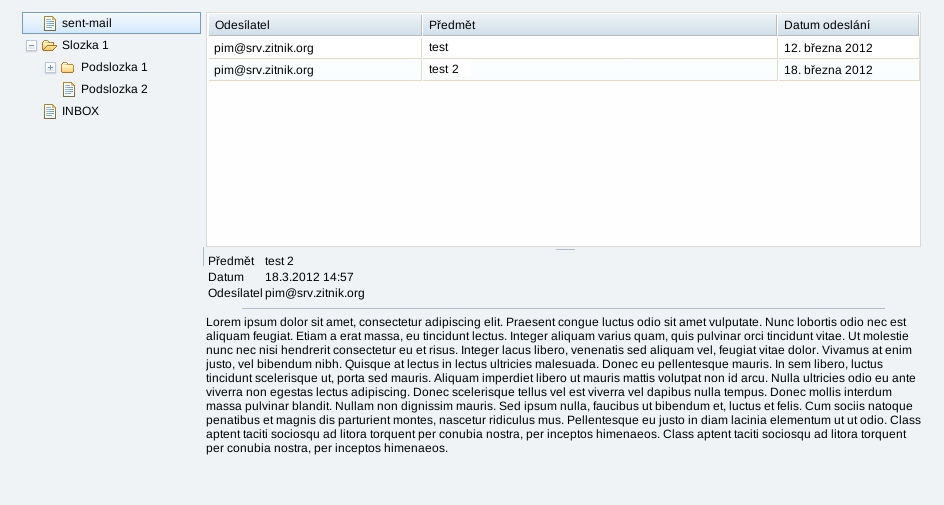
\includegraphics[width=\textwidth]{../mailScreen.png} 

Pro každý účet je zobrazen strom složek, využívající komponentu dijit.Tree. Komponenta dijit.Tree vyžaduje datový modelu, který je implementován ve třídě app.ForestStoreModel. Tento datový model zajišťuje dynamické načítání jednotlivých větví stromu ze serveru, takže strom nemusí být načtěn v~paměti celý.
Model také poskytuje informace o~tom, která položka ve stromu má další potomky. Toho využívá dijit.Tree k~vykreslení rozbalovací struktury.

Seznam emailů je vázán na vybranou složku ve stromu. Ve výchozím stavu se automaticky zobrazuje \uv{INBOX}. Zobrazovací prvek pro výpis emailů je dojox.grid.DataGrid, který představuje tabulku s~předem defonovanými sloupci. Jako všechny DoJo widgety pracující s~daty vyžaduje instanci DoJo store třídy - v~tomto případě zase JsonStore.

Zobrazování samotné emailové zprávy zprostředkovává instance třídy DataForm, která si stáhne kompletní rozparsovanou zprávu pomocí JsonStore a~pouze vykreslí HTML šablonu.

Odesílání emailových zpráv funguje obdobně. Třída app.gui.mail.NewMail vykresluje základní uživatelské rozhraní pro vytváření zpráv.
Zobrazuje 3 vstupní prvky - přijemce, předmět a~HTML editor pro samotnou zprávu. Vstupní prvek příjemce je dijit.form.ComboBox, který funguje jako našeptávač. Tento našeptávač pomocí JsonStore komunikuje se serverovým modulem Contacts, který prohledává kontakty uživatele a~případně automaticky nabízí a~doplňuje emailové adresy do vstupního prvku.

Při odesílání emailové zprávy se volá na serveru metoda sendMail() z~modulu mail/MailMessage, která využívá jednoduchý SMTP přístup popsaný v~kapitole \ref{sec:mailClient}

\section{Závěr}
\label{sec:Conclusion}
Výsledkem této bakalářské práce je plně funkční systém splňující základní požadavky na správu osobních informací.
Aplikace je rozdělena na dvě nezávislé části - server a~klient, což umožňuje implementaci dalších klienstkých aplikací pro různé platformy a~použití.

Pro úspěšnou realizaci této práce byl zapotřebí především dobrý návrh a~architektura celého systému. Dále také byla nutná dobrá znalost použitých technologií, především programovacích jazyků Python a~JavaScript včetně frameworku DoJo.

Realizace byla pro mne přínosná v~podobě nově získaných znalostí a~problematiky univerzální komunikace mezi klientem a~serverem, zpracování informací a~tvorbě uživatel\-ských rozhraní v~internetovém prohlížeči.

Dokončením bakalářské práce vývoj PIM aplikace nekončí, bude se nadále rozvíjet a~především bude snaha o~rozšíření uživatelské komunity. Do budoucna je v~plánu dále rozšiřovat a~vyvíjet obě části, především serverovou stranu pro sdílení informací mezi více uživateli a~aplikace pro systém Android. To by mělo výrazně přispět k~rozšíření tohoto systému mezi uživatele mobilních telefonů.



\bigskip
\begin{flushright}
Jan Žitník
\end{flushright}


\begin{thebibliography}{99}

%Python
\bibitem{svec-letajici-cirkus}Švec, Jan,
\textit {Seriál Python - Létajíc cirkus} Root.cz : informace nejen ze světa Linuxu [online]. Verze 1.0. 2001 [cit. 2011-04-23]. Létající cirkus. Dostupné z~WWW: http://www.root.cz/clanky/letajici-cirkus/


\bibitem{python-kniha}Harms, Daryl - McDonald, Kenneth
\textit {Začínáme programovat v~jazyce Python}
Praha : Computer Press 2008.


%JavaScript
\bibitem{javascript-kniha}Zakas, Nicholas Z.,
\textit{JavaScript pro webové vývojáře}
Praha : Computer Press 2009

\bibitem{javascript-definice}
\textit{Adaptic}
Co je to JavaScript [online]. 2012. Dostupné z~URL:
$<$http://www.adaptic.cz/znalosti/slovnicek/javascript$>$

\bibitem{javascript-json}
\textit{Wikipedie - Otevřená encyklopedie}
JavaScript Object Notation [online]. 2012. Dostupné z~URL:
$<$http://cs.wikipedia.org/wiki/JavaScript\_Object\_Notation$>$

%postgres
\bibitem{postgres-kniha}Bruce, Momjian
\textit{PostgreSQL - praktický průvodce}
Praha : Computer Press 2003

\bibitem{postgres-wiki}
\textit{Wikipedie - Otevřená encyklopedie}
PostgreSQL [online]. 2012. Dostupné z~URL:
$<$http://cs.wikipedia.org/wiki/PostgreSQL$>$

%mail
\bibitem{imap-wiki}
\textit{Wikipedie - Otevřená encyklopedie}
IMAP [online]. 2012. Dostupné z~URL:
$<$http://cs.wikipedia.org/wiki/Internet\_Message\_Access\_Protocol$>$

\bibitem{smtp-wiki}
\textit{Wikipedie - Otevřená encyklopedie}
SMTP [online]. 2012. Dostupné z~URL:
$<$http://cs.wikipedia.org/wiki/Simple\_Mail\_Transfer\_Protocol$>$


%dojo
\bibitem{dojo-guide}Russell, Matthew A.
\textit{Dojo: The Definitive Guide} 
Farnham : O'Reilly, 2008.

\bibitem{json-rfc}Crockford, D.,
\textit{RFC 4627} The application/json Media Type for JavaScript Object Notation (JSON)
http://tools.ietf.org/html/rfc4627

\bibitem{imap-rfc}Crispin, M.,
\textit{RFC 3501} INTERNET MESSAGE ACCESS PROTOCOL - VERSION 4rev1
University of Washington 2003

\bibitem{smtp-rfc}Klensin, J.
\textit{RFC 2821} Simple Mail Transfer Protocol
AT\&T Laboratories 2001


\end{thebibliography}

\appendix
\section{Obrázky aplikace}

\InsertFigure{../screens/screen1.png}{\textwidth}{Dashboard}

\InsertFigure{../screens/screen2.png}{\textwidth}{Měsíční pohled}

\InsertFigure{../screens/screen3.png}{\textwidth}{Poznámky}

\InsertFigure{../screens/screen4.png}{\textwidth}{Kontakty}

\InsertFigure{../screens/screen5.png}{\textwidth}{RSS feedy}

\InsertFigure{../screens/screen6.png}{\textwidth}{Týdenní pohled a drag\&drop}

\InsertFigure{../screens/screen7.png}{\textwidth}{Vytváření nové události}



\clearpage

\end{document}
